
% \section{Introduction}
%% DEMOCRACY has problems and bureaucratic solutions
%Large democracies face two big problems. First, they are vulnerable to fleeting passions and demagogues. To combat this, many decisions are left to experts who, ideally, exercise judgment loosely guided by the public. Second, everyone cannot vote on every decision. We thus delegate power to representatives (who then delegate it to deputies), create temporary mini-publics, and solicit input from those most affected or moved by a public decision.\footnote{As imagined by \citet{Dahl1989}, mini-publics are representative, selected at random, and deliberative. Besides juries, however, randomly selected deliberative bodies are rare. Instead, citizens more often engage in government decisions when given opportunities to opt-in, such as hearings, petitions, and public comment periods. These mechanisms of engagement generate a different, more contentious flavor of public input than the discourse imagined by scholars who focus on deliberation.} Most policy is then made by bureaucrats, supposedly guided indirectly through elected representatives and directly by limited public input (mostly limited to more contentious policy debates).

% Both of these problems converge in the bureaucracy, run by experts who are deputized by elected officials (or by their deputy's deputy's deputy) and with procedures that create opportunities for public input. It is far from clear how bureaucratic decisions are to balance expertise, accountability to elected officials, and responsiveness to public input in decisionmaking. 


% \subsection{Why study rulemaking?}
% \section{The Importance of Studying Rulemaking}
% Mobilization may increasingly target rulemaking because it is how most policy in the U.S. is now made. 

% rulemaking matters 
With the rise of the administrative state, U.S. federal agencies have become a major site of policymaking and political conflict. By some estimates, upward of 90\% of legally binding U.S. federal policy is now written by agencies. Agency rules are revised much more frequently than statutory law \citep{Wagner2017} and in the years or decades between legislative enactments, federal agencies make legally-binding rules interpreting and reinterpreting old statutes to address emerging issues and priorities. %Ninety percent of new policy that carries the force of law is now made in the bureaucracy rather than in Congress \citep{West2013}.\footnote{I use policy, law, and regulation as nested concepts. My methods generally apply to all policy texts whether they carry the force of law or not. Many public and private organizations, including agencies, have policy statements that are not legally binding. My empirical subject is rules that do carry the force of law based on some authorizing legislation. I use rule (a more technical term) and regulation (a more colloquial term) interchangeably.}
Examples are striking: The effect of the Dodd-Frank Wall Street Reform and Consumer Protection Act was largely unknown until the specific regulations were written, and it continues to change as these rules are revised. 
Congress authorizes billions in farm subsidies and leases for public lands, but who gets them depends on agency policy. In the decades since the last major environmental legislation, agencies have written thousands of pages of new environmental regulations and thousands more changing tack under each new administration. These revisions significantly shape lives and fortunes. For example, in 2006, citing the authority of statutes last amended in the 1950s, the Justice Department's Bureau of Prisons proposed a rule restricting eligibility for parole. In 2016, the Bureau withdrew this rule and announced it would require fewer contracts with private prison companies, precipitating a 50\% loss of industry stock value. Six months later, a new attorney general announced these policies would again be reversed, leading to a 130\% increase in industry stock value. %Like many rulemaking debates, industry and advocacy groups spent millions of dollars lobbying on this issue. Few rulemakings, however, receive this level of public and presidential attention. In the majority of rulemakings, few participate, and we do not know the extent to which participants get what they lobby for.% (but see Yackee and Yackee 2006)
Agency rulemaking matters.

% democracy interbranch relations and autonomy
Less clear, however, is how the new centrality of agency rulemaking fits with democracy. In addition the bureaucracy's complex relationships with the president and Congress, agencies have complex and poorly understood relationships with the public and advocacy groups. Relationships with constituent groups may even provide agencies with a degree of ``autonomy'' from their official principals \citep{Carpenter2001}. % CITE {Yackee2019}.

%\paragraph{Expertise, accountability, and participation.} 
Debates over the proper roles of bureaucratic expertise, congressional delegation, and limited public input converge in bureaucratic policymaking. Bureaucratic policymaking involves expert judgment, accountability to elected officials, and be responsive to public input. %\footnote{ Notice and comment rulemaking is the main focus of political science scholarship on bureaucratic policymaking in the United States \citep{West2015, Yackee2006JPART, Yackee2010PSQ, Kerwin2011} } 
Processes like public comment periods, where agencies must solicit public input on draft policies, are said to produce valuable technical information \citep{Yackee2006JPART, Nelson2012}, oversight opportunities \citep{Balla1998, Mccubbins1984}, and democratic legitimacy \citep{Croley2003, Rosenbloom2003}. There is no normative consensus on how to rank or merge these goals \citep{Wilson1967, Wilson1989, Carrigan2017}. Procedures requiring agencies to solicit public input and the justification of these procedures cite all three aims. For example, these various goals are evident in the Administrative Conference of the United States (ACUS) Proposed Recommendation on Public Engagement in Rulemaking, which asserts that ``The opportunity for public engagement is vital to the rulemaking process, permitting agencies to obtain more comprehensive information, enhance the legitimacy and accountability of their decisions, and enhance public support for their rules'' \citep{ACUS2018}. Public comment periods are purported to simultaneously produce technical information, accountability to elected officials, and responsiveness to public demands.

% gap
Yet, legitimacy, accountability, public support, and, especially, collecting information depend not just on the opportunity to engage but actual engagement \citep{Herz2018}, and we know surprisingly little about the vast majority of public comments (i.e., those submitted by ordinary people as part of a public pressure campaign) and the role that this kind of input may or may not play in rulemaking.


% DEFINITION
%\paragraph{Defining mass engagement}
Political scientists often define civic engagement as writing to government officials, signing petitions, attending hearings, attending protests, or donating to a political campaign \citep{Verba1987}. While donating is more common in electoral politics, activists frequently target agency policymaking with letter-writing campaigns, petitions, protests, and mobilizing people to attend hearings. 
% I suspect that mass commenting is driven by the same privileged populations known to engage in other civic activities. 
% Does it work? If so, by what mechanisms?
Contrary to the common assumption that mass engagement emerges organically, it is almost always mobilized by an organization that also engages in sophisticated lobbying or coordination with such an organization.\footnote{Following the conventional terms ``mass comment campaign'' and ``public engagement,'' I call the general phenomenon ``mass engagement'' resulting from a ``mass mobilization campaign'' to distinguish the magnitude of civic engagement. By mass engagement, I mean that thousands of people beyond professional policy influencers engage. In my empirical context of agency rulemaking, I define mass engagement as more than 1000 public comments or 100 identical comments, plausibly indicating a mobilization effort. This differs from the Environmental Protection Agency's definition of mass comment campaign as two or more identical comments. In the results below, I use an intermediate category---``small batch''---comments to describe identical comments numbering less than 100}  %\footnote{
As \citet{SantAmbrogio2018} conclude ``The `mass comments' occasionally submitted in great volume in highly salient rulemakings are one of the more vexing challenges facing agencies in recent years. These comments are typically the result of orchestrated campaigns by advocacy groups to persuade members or other like-minded individuals to express support for or opposition to an agency's proposed rule.'' % While some dismiss mass comments as spam, I take public expressions of support or opposition seriously as political participation where people aim to communicate demands to public officials.
% To better understand this vexing challenge, 
% existing models cant explain gap

While practitioners and administrative law scholars have long pondered what to make of mass commenting, political scientists have had surprisingly little to say about this kind of civic participation. 
The contentious politics that inspire the majority of public comments have no place in leading models of bureaucratic policymaking and have largely been ignored by political scientists.\footnote{ 
But see \citet{Yackee2015JPART}, who surveys commenters, finding that members of the public believe their comments matter, even though powerful groups have more influence; \citet{Cuellar2005}, who examines public input on three rules, finding that ordinary people made up the majority of commenters, which, he argues, ``shows at least some potential demand among the mass public for a seat at the table in the regulatory process''; \citet{Moore2017}, who identifies several key predictors of which rules receive more comments; \citet{Shapiro2008} who studied nine rules, finding the more complex but lower-salience rules with more comments were also the ones that changed; and \citet{Balla2018} and \citet{Potter2017}, who find mass comment campaigns driving significant participation of ordinary people in EPA rulemaking. 
}
% pol sci lit 
Instead, models focus on how agencies either learn about policy problems, negotiate or avoid accountability to various principals, or balance interest-group demands.\footnote{
On learning, see \citet{Kerwin2011} and empirical studies by \citet{yackee2012}, \citet{Cook2017}, \citep{Gordon2018}, and \citet{Walters2019}. See \citet{Gailmard2017} and \citet{Libgober2018} for information-based models where comments reveal information to the agency. 

On accountability to elected officials, see  \citet{Furlong1997}, \citet{Nou2016}, \citet{Potter2016}, \citet{Woods2018}, and \citet{Yackee2009RegGov}. See \cite{Gailmard2012} for a review of formal models of oversight.
%\citet{Epstein1994} propose a model where delegation depends on how much information and veto power principals have.
Especially relevant to my analysis of the effects of mass mobilization on oversight, \citet{Potter2014dis} develops a signaling model where agencies propose and principals veto rules depending, in part, on their beliefs about interest group preferences. 

On interest group balancing see \citet{Yackee2006JOP},  \citet{Yackee2006JPART}, and \citet{Kerwin2011}. A key assumption of Libgober's (2018) model is that bureaucrats have a distribution of preferences over interest group positions, about which they are uncertain unless groups reveal their preferences through commenting.
} 
% SOPHISTICATED LOBBYING
% Influence in rulemaking is sophisticated lobbying efforts of powerful interest groups, whose role in shaping policy has been theoretically developed and empirically tested.

\paragraph{Most scholars are skeptical that ordinary people can affect rulemaking.} Foundational scholarship on rulemaking by \citet{Furlong2004}, \citet{Furlong1997, Furlong1998}, and \citet{Kerwin2011} focuses on interest group lobbying. To the extent scholars address the input of ordinary people %---i.e., not professional policy influencers---
at all, both existing theory and empirical scholarship suggest skepticism that it matters. (By ``ordinary'' people, I simply mean people who are not professional policy-influencers, not that these politically-engaged people are demographically representative of the broader public.)
% REREAD BERRY
% \citet{Berry1999TheGroups} argues that mass engagement occurs too late in the policy process to be effective compared to insiders who shape agendas and alternatives. 
Empirical scholarship finds that economic elites and business groups dominate American politics in general \citep{Gilens2014} and rulemaking in particular. %Perhaps this is unsurprising. 
% gap - REPRESENTATION - don't know who is represented
While some are optimistic that requirements for agencies to solicit and respond to public comments on proposed rules allow ``civil society'' to provide public oversight \citep{Michaels2015, Metzger2010}, most studies find that participants in rulemaking often represent elites and business interests \citep{Seifter2016UCLA, Crow2015, Wagner2011, West2009, Yackee2006JOP, Yackee2006JPART, Golden1998, Haeder2015, Cook2017}.%, Libgober2018MeetingsDodd-Frank}. %Balla2011,Yackee2012

From a strategic perspective, agency officials are not directly accountable to voters. And even if organized groups do supplement congressional and judicial checks on executive power, the groups that participate in rulemaking represent only certain (if any) segments of the public and may not represent them well \citep{Seifter2016UCLA}. Scholars are thus skeptical about rulemaking as a site for collective action the ability of most people to participate.
% From a science-based policy perspective, average citizens signing form letters provide no new information to policymakers. 
As a result, mass comment campaigns are dismissed as epiphenomenal to bargaining with principals or interest groups. Indeed, almost all empirical studies of rulemaking discard unsophisticated comments from ordinary people, as evident from a comprehensive review of scholarship on ``The Politics of Rulemaking'' by \citet{Yackee2018}, who finds skepticism about citizen comments, but no studies analyzing mass mobilization as a lobbying tactic:
\begin{quote}
    ``\citet{Kerwin2011} point out that a citizen must know not only that a regulation is being formulated but also how and when to participate. This is a high bar for most Americans. Second, to be influential during rulemaking, commenters may require resources and technical expertise. As \citet{Epstein2014} suggest, agency rule-writers--who are often chosen because of their technical or policy-specific expertise--privilege the type of data-driven arguments and reasoning that are not common to citizen comments.
    %When taken together, these factors suggest why interest group lobbying may occur at a higher rate than citizen lobbying. In short, interest groups are better able to afford the costs of regulatory participation \citep{Yackee2006BJPS}. This may come as no surprise to students of interest group politics, who have long known the difficulty of collective action across citizens \citep{Olson1965}, as well as the problems associated with mobilizing citizen groups, who have no ready-made constituency and no easy sources of political funding \citep{Walker1991}.
    '' (p. 10)
     \end{quote}
For any particular lay commenter, this conclusion seems inescapable. But groups do occasionally mobilize, usually behind a more sophisticated lobbying effort. %Are ordinary people still powerless when mobilized in large numbers?
%Despite the skepticism assumed by scholars, \citet{Yackee2015JPART} finds that ordinary participants strongly believe that their comments matter, even if they see businesses as more influential.
Without systematic understanding and study of public participation, it is difficult to adjudicate such questions about how processes like public comment periods may enhance or undermine various democratic ideals.

% but so many mass comments
This scholarly oversight is surprising given that most people are only aware of rulemaking when it is the target of a high-profile mass mobilization campaign.\footnote{
Some of the most contentious recent public controversies involve bureaucratic policymaking. For example, along with 50 thousand protesters in Washington D.C., the State Department Received 1.2 million comments on the Environmental Impact Statement for the Keystone Pipeline. Similarly, along with the thousands of protesters supporting the Standing Rock Sioux protest to the Dakota Access Pipeline, the Army Corps of Engineers received hundreds of thousands of comments. Alongside protest actions that included shutting down many websites, the Federal Communications Commission's open internet rule received 22 million comments. While some of these comments appear to be fake, the scale of public engagement is remarkable given how little attention political scientists have paid to it. Fake public comments also raise the question of why an organization would bother to generate fake public input if it did not matter, as its omission from theories of bureaucratic policymaking would seem to imply. %On each of these issues, advocacy activity has been followed by legislative or executive action.
} 
While most rules receive little attention, the ease of online mobilizing and commenting has, like other forms of participation \citep{Boulianne2018}, created exponential increases in the number of rules in which thousands and even millions of people engage (see Figure \ref{fig:comments}; note that comments per rule are on a logarithmic scale).\footnote{
Proposed rules that have attracted the most public attention have been published by the Federal Communications Commission (FCC, omitted from this plot), the Environmental Protection Agency (EPA), the Department of Interior (DOI), the Bureau of Ocean Energy Management (BOEM), the Consumer Financial Protection Bureau (CFPB), and Fish and Wildlife Service (FWS).
}
Occasionally, a large number of people are paying attention. These bursts of civic participation may affect rulemaking \citep{Coglianese2001}, but this intuition has yet to be tested.

% advertises it as democracy 
The general failure to explain or account for mass engagement in rulemaking is also striking in light of how agencies advertise public comment periods as an opportunity for a voice in government decisions.\footnote{
% FOCUS
I focus on public comments in rulemaking, but the theories and methods here may also apply to other kinds of political engagement such as through social media or protests as well as to other political decisions, including state-level rulemaking. Social media engagement may be especially important if agencies implement the recommendations of \citet{ACUS2018} that ``Agencies should consider using social media before or in connection with direct final rulemaking to quickly identify whether there are significant or meaningful objections'' (p. 34). 
} 
Big red letters across the top of the Regulations.gov homepage solicit visitors to ``Make a difference. Submit your comments and let your voice be heard'' (Figure \ref{fig:regs.gov}). A blue ``Comment Now!'' button accompanies a short description of each draft policy and pending agency action. 
Another invitation at the bottom of the page reads ``Participate today!''
Public commenting on proposed agency rules is described as ``an important part of democracy'' (WSJ 2017), the ``often held out as the purest example of participatory democracy in actual American governance'' \citep{Herz2016}. \citet{Rossi1997} finds that ``courts, Congress, and scholars have elevated participation [in rulemaking] to a sacrosanct status...greater participation is generally viewed as contributing to the democracy.'' % Is it?
Despite much debate about the theoretical import and possible reforms, the bulk of public comments have yet to be studied.

\begin{figure}[t]
    \centering
    \caption{Regulations.gov Solicits Public Comments on Draft Agency Rules}
    \label{fig:regs.gov}
    
    
\includegraphics[width= 6.5in]{regulations-header.png}
\end{figure}

\begin{figure}
\caption{Comments on Proposed Rules per Year (left) and per Rule (right) posted on regulations.gov}
\centering
%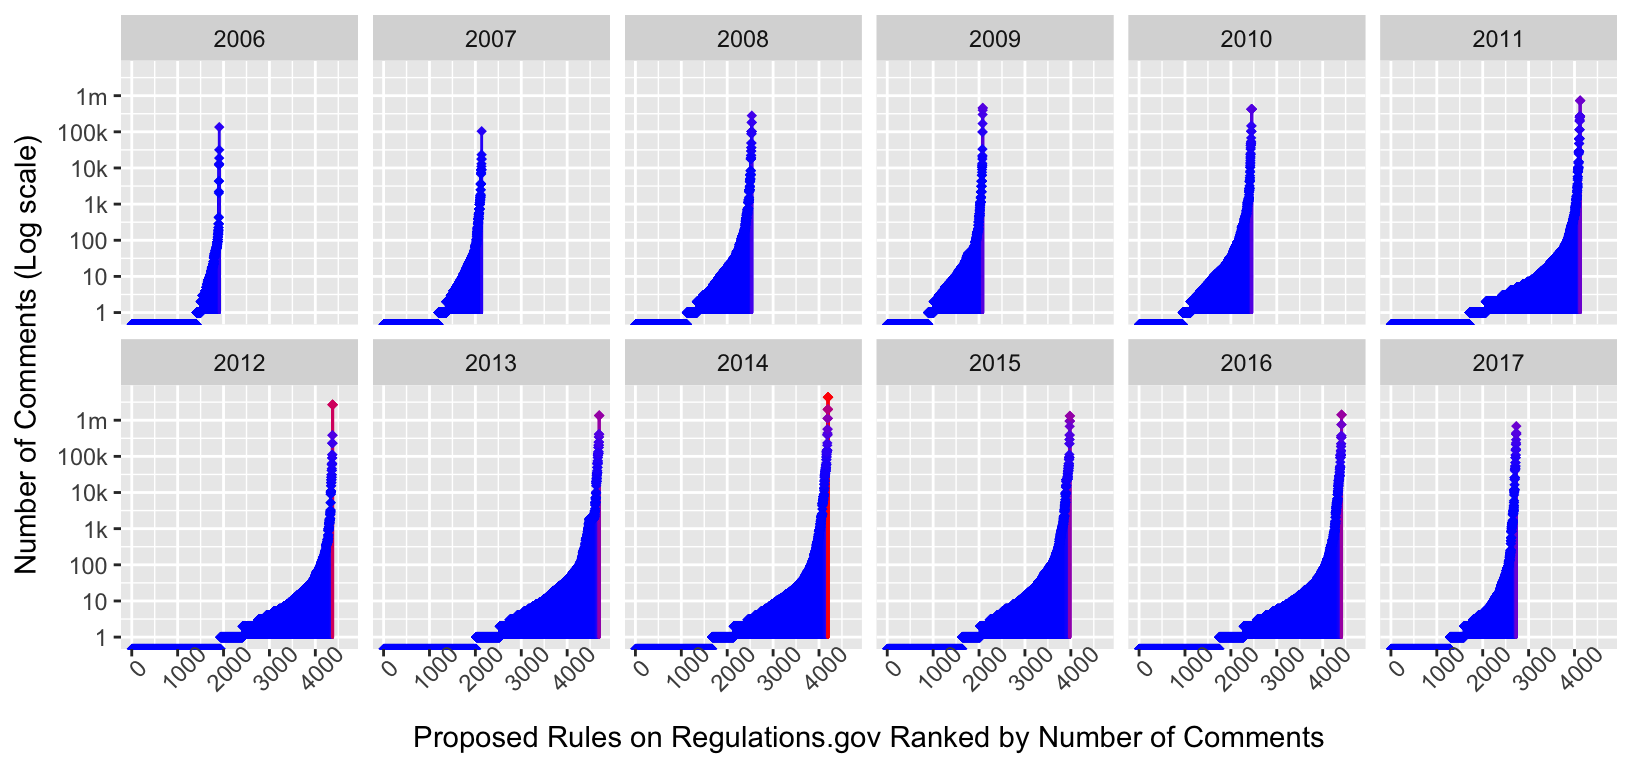
\includegraphics[height= 2.5in]{Figs/comments-per-year-1.png}
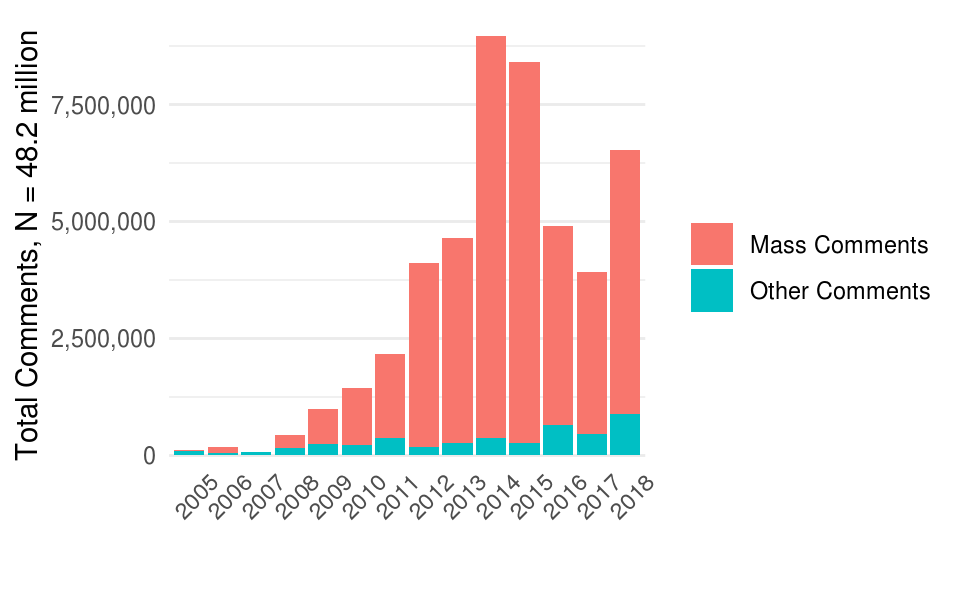
\includegraphics[height= 2.4in]{Figs/comments-mass-vs-unique-1.png}
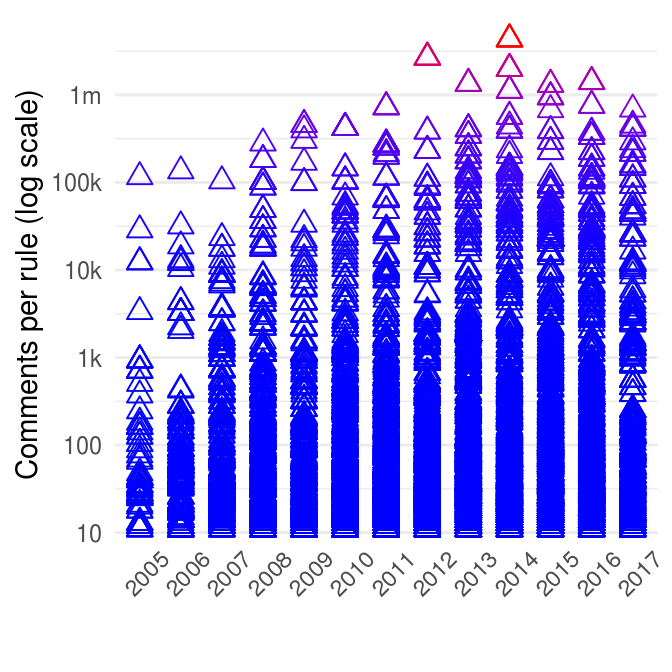
\includegraphics[height= 2.4in]{Figs/rules-comments-per-year-1.png}
\label{fig:comments}
\end{figure}



%It is even less clear whether actions by average citizens make a difference in agency policymaking. Many may believe that they do, but the mechanisms are not obvious. Indeed letter writing and other forms of mass mobilization do not have a clear place in political scientists' theories of bureaucratic politics. This lack of scholarship may be the result of both a general suspicion, rooted in certain theories of strategic behavior, that mass politics affects unelected career officials as well as a normative assumption that policy ``implementation'' is no place for contentious politics. Neither the bureaucrat who asserts that rules are the result of scientific analysis nor the political scientist who asserts that rules are the result of bureaucrats strategically selecting their most preferred policy within institutional constraints explain why an agency would receive millions of public comments or why they would matter.











% % LEGAL SCHOLARS' DEBATES 
In contrast to political scientists, legal scholars have long debated what to make of mass commenting in rulemaking. Many focus on reforms to help agencies collect more useful information \citep{Farina2011, Farina2014, Rauch2016}. In 2018, ``Public engagement'' was main project of the Administrative Conference of the United States (ACUS) committee on Rulemaking: %\href{https://www.acus.gov/research-projects/public-engagement-rulemaking}
{The project} 
\begin{quote}``explores agency strategies to enhance public engagement prior to and during informal rulemaking. It seeks to ensure that agencies invest resources in a way that maximizes the probability that rulewriters obtain high-quality public information.'' 
\end{quote} 
Among other things, this committee is debating how best to gather ``quality public information,'' how ``to get new people/groups into the real or virtual room'' \citep{Farina2018}, and whether broad engagement is even desirable on all rules \citep{White2018}. 

Administrative law scholars have explored these questions theoretically for decades, but only a few offer empirical analysis. \citet{Mendelson2011} finds that agencies often discard non-technical comments but argues that they should be given more weight. Others worry that mass commenting distracts agencies from good policy and the broader public interest \citep{Coglianese2006}. \citet[p. 112]{Farina2012} claims that ``[Mass] comments typically are neither factually informative nor reliable indicators of citizens’ informed value preferences.'' Some even call them ``spam'' \citep{Balla2018, Novek2004}. In this prevailing view, ``high-quality'' and ``relevant'' mean novel technical information, not opinions. \citet[p. 208]{Herz2016} concludes ``The goal of e-rulemaking is to more fully capture such credible, specific, and relevant information, not to solicit the views of random, self-nominating members of the public.'' Similarly,  \citet[p. 4]{Epstein2014} dismiss mass comments as ``effectively, votes rather than informational or analytical contributions. Rulemaking agencies are legally required to make policy decisions based on fact-based, reasoned analysis rather than majority sentiment; hence, even hundreds of thousands of such comments have little value in the rulemaking process.''  Notably, the ACUS draft recommendations on ``Mass and Fake Comments in Agency Rulemaking'' suggests that ``effective comments'' give ``reasons rather than just reactions'' \citep[p. 33]{ACUS2018}. If true, most public reactions to proposed rules such as those expressed in mass comments would have no effect in rulemaking. 

Early optimism among legal scholars that the internet would ``change everything'' \citep{Johnson1998} and that ``cyberdemocracy''  would enable more deliberative rulemaking has faded.  
While commenting and mobilizing others to comment has become easier, \citet{Coglianese2006} finds that little else has changed. %\citet{Rossi1997} even suggests that public comment processes should be largely eliminated.
The prediction that the internet would primarily facilitate more of the same kind of engagement among the like-minded (i.e. mass-commenting) \citep{Sunstein2001} has largely been correct. In this sense, the ``quality'' of discourse has not improved.

Even scholars who suggest reforms aimed at ``regulatory democracy'' aim to increase the ``sophistication'' of ordinary peoples' comments \citep{Cuellar2014, Johnson2013}. For example, \citet{Novek2004}  is critical of ``notice and spam,'' arguing instead for ``participative practices---methods for `doing democracy' that build the skills and capacity necessary for citizens, experts, and organizations to speak and to be heard. Rulemaking, after all, is a communicative process involving a dialogue between regulators and those affected by regulation" \citet[p. 3]{Noveck2005}.

This scholarship has improved the theory and practice of policy learning in rulemaking. But a focus on sophisticated deliberation and technical information overlooks the potential role of political information.\footnote{But see the below review of insights from \citet{Golden1998}, \citet{Nelson2012}, \citet{Rauch2016}, and \citet{Potter2017} on political information and \citet{Reich1966} and \citet{Seifter2016UCLA} on representation.} Whereas administrative law scholars have focused on ``how technology can connect the expertise of the many to the power of the few'' \citep{Noveck2009}, I ask whether it may also connect the power of the many to the decisions of the few. 

While ``ordinary'' members of the public may occasionally provide novel and useful technical information to expert bureaucrats, such sophisticated means of influencing policy are out of reach for the vast majority of people. Thus, to investigate the potential role of ordinary people in bureaucratic politics I look elsewhere---not because ordinary people never provide novel and useful technical information, but because this is not how most people attempt to influence policy, nor, I argue, how we should expect ordinary people to have influence.

Most public comments are, in fact, of the flavor suggested by the solicitations on Regulation.gov---ordinary people voicing opinions on a proposed policy. They do not provide useful technical information or suggest specific edits to policy texts like the interest group comments that have thus far captured the attention of political scientists. If they add information to rulemaking, it is a different, more political flavor of information.  Indeed as Figure \ref{fig:comments} shows, every year since 2008, most people who comment on draft regulations have done so as a result of an interest group's campaign.\footnote{At least for agencies participating in regulations.gov. See sections \ref{whyMail-methods} and \ref{whyMail-results} for my definition and methods for identifying mass comments.} 
Public engagement in rulemaking is highly clustered on a few rules made salient by these campaigns. It is plausible that, at least some of the time, such campaigns aim to influence policy. It is also plausible that thousands of people engaging may alter the politics of these policy processes, but this hypothesis remains untested. Indeed, we have much to understand about the causes and effects of these campaigns before we are in a position to ask if they are a mechanism for %social movement 
groups to influence policy. Most critically, we must understand who mobilizes and why.

The kind of politics created by mass engagement has a few notable features. It is contentious; most ordinary people are not engaging in deliberation, they are simply making demands. Importantly, however, processes like public comment periods channel contentious demands into institutionalized policy processes rather than undermining them. % cite Ian Henning? 
Mass commenting may also, in a sense, expand participation.\footnote{
If defining ``political participation'' as ``acts aimed at influencing governmental decisions \citep[p. 2]{Verba1987}, signing a petition or mass comment counts. However, some consider true participation to be deliberative, which mass commenting is not. Other requirements, that participation is ``genuine,'' ``informed,'' or ``reasoned'' are more difficult to assess. % Normative, more participation is generally understood as more democracy, but critics on the left worry that people may be socialized to work against their own interests {Bardrach and Baratz 1963} and critics on the right doubt whether people are capable of knowing their best interest {Lippman}
Normative theorists may debate whether deliberation among a small number of people is preferable to a large number of people simply expressing their preferences, but empirically, public participation in bureaucratic policymaking is much more the latter.
} 
Surely, those who opt in are far from representative of the broader public \citep{Verba1987}, but in many ways, they must be more representative than the handful of political insiders who participate in most policy processes. If the usual participants have ``an upper-class accent'' as \citet{Schattschneider1942} put it, adding thousands of more voices may dilute this bias. This likely depends on how people are mobilized. If mass engagement is mobilized by the usual participants to create an impression of public support, it may even legitimize the demands of powerful interest groups. In short, the politics of rulemaking created by mass engagement is much more contentious than most rulemakings, but also much more institutionalized than most contentious politics. Mass engagement in rulemaking thus presents a novel context to examine the consequences of broader engagement in typically insider-dominated policymaking and how public participation may condition how political decisions are made. 











%%%%%%%%%%%%%%%%%%%%%%%%%%%%%%%%%%%%%







% MODEL - regulator is uncertain about backlash 
% org may reveal 
% people react to losses more than gains 
% 262 in 6th edition - useful thing in identifying diffuse interests - though they may not be opposed before - they may mobilize after 



 %While the theory that I assemble attempts to describe the relationship between mass mobilization and agency decisionmaking in general, my empirical focus is on the role of organized campaigns targeting notice-and-comment rulemaking processes, with particular attention to environmental and financial regulation.




%  1946 Administrative Procedure Act (APA), which includes any “agency statement of general or particular applicability and future effect designed to ...interpret, or prescribe law or policy” [U.S.C. §551(4) (1994)].





